In this problem, the discrete time feedback is tested on the nonlinear model. The controller has been implemented on the SIMULINK model of the nonlinear system (see figure \ref{fig:modelp17} in Appendix \ref{AppP17}).

The state responses to $x_{ref}$ has been plotted figure \ref{fig:p17time} in the time domain and figure \ref{fig:p17freq} in the frequency domain. 

\begin{figure}[H]
 \centering 
 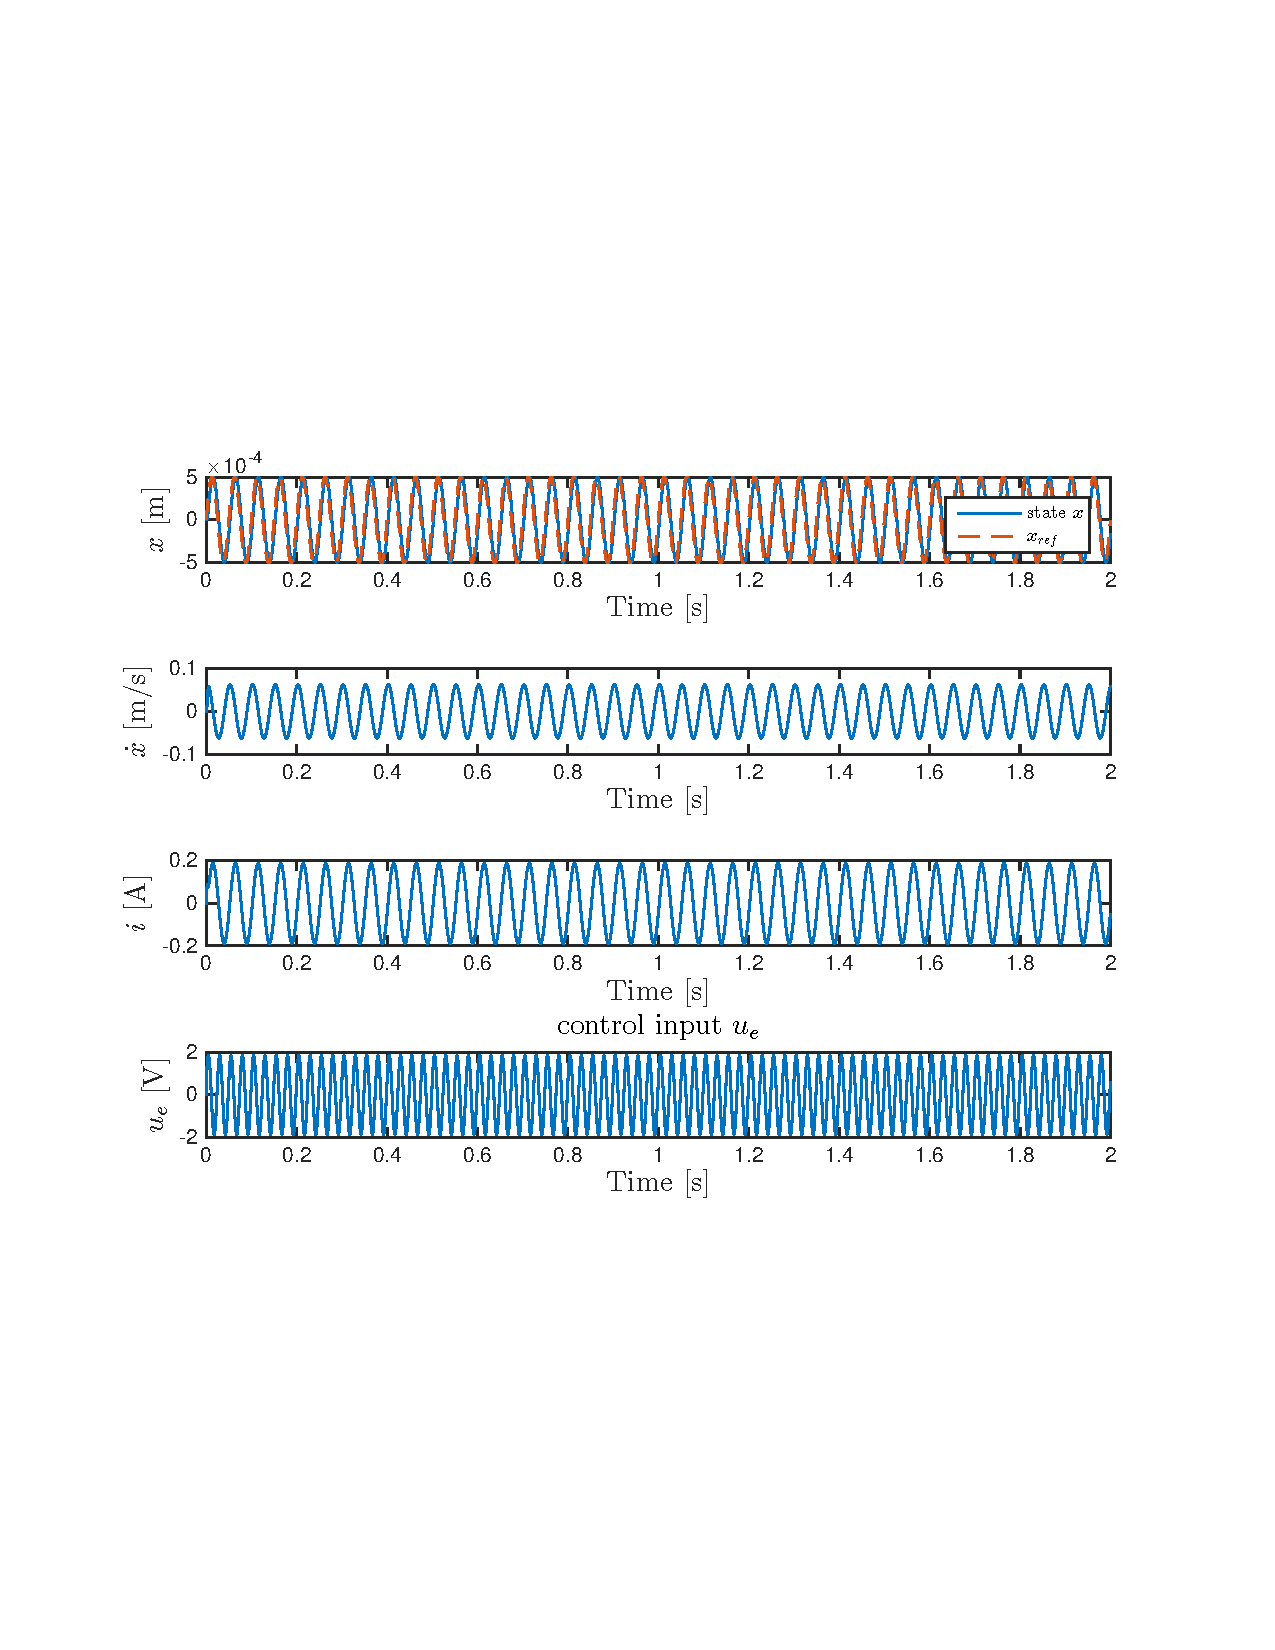
\includegraphics[trim=0cm 7cm 0cm 7cm, clip=true, totalheight=0.35\textheight, angle=0]{figures/p17time.pdf}
 \caption{$u_e$ and state responses to $x_{ref}$ with $Ax = 0.0005\ m$ using the controller on the nonlinear model.}
 \label{fig:p17time}
\end{figure}

\begin{figure}[H]
 \centering 
 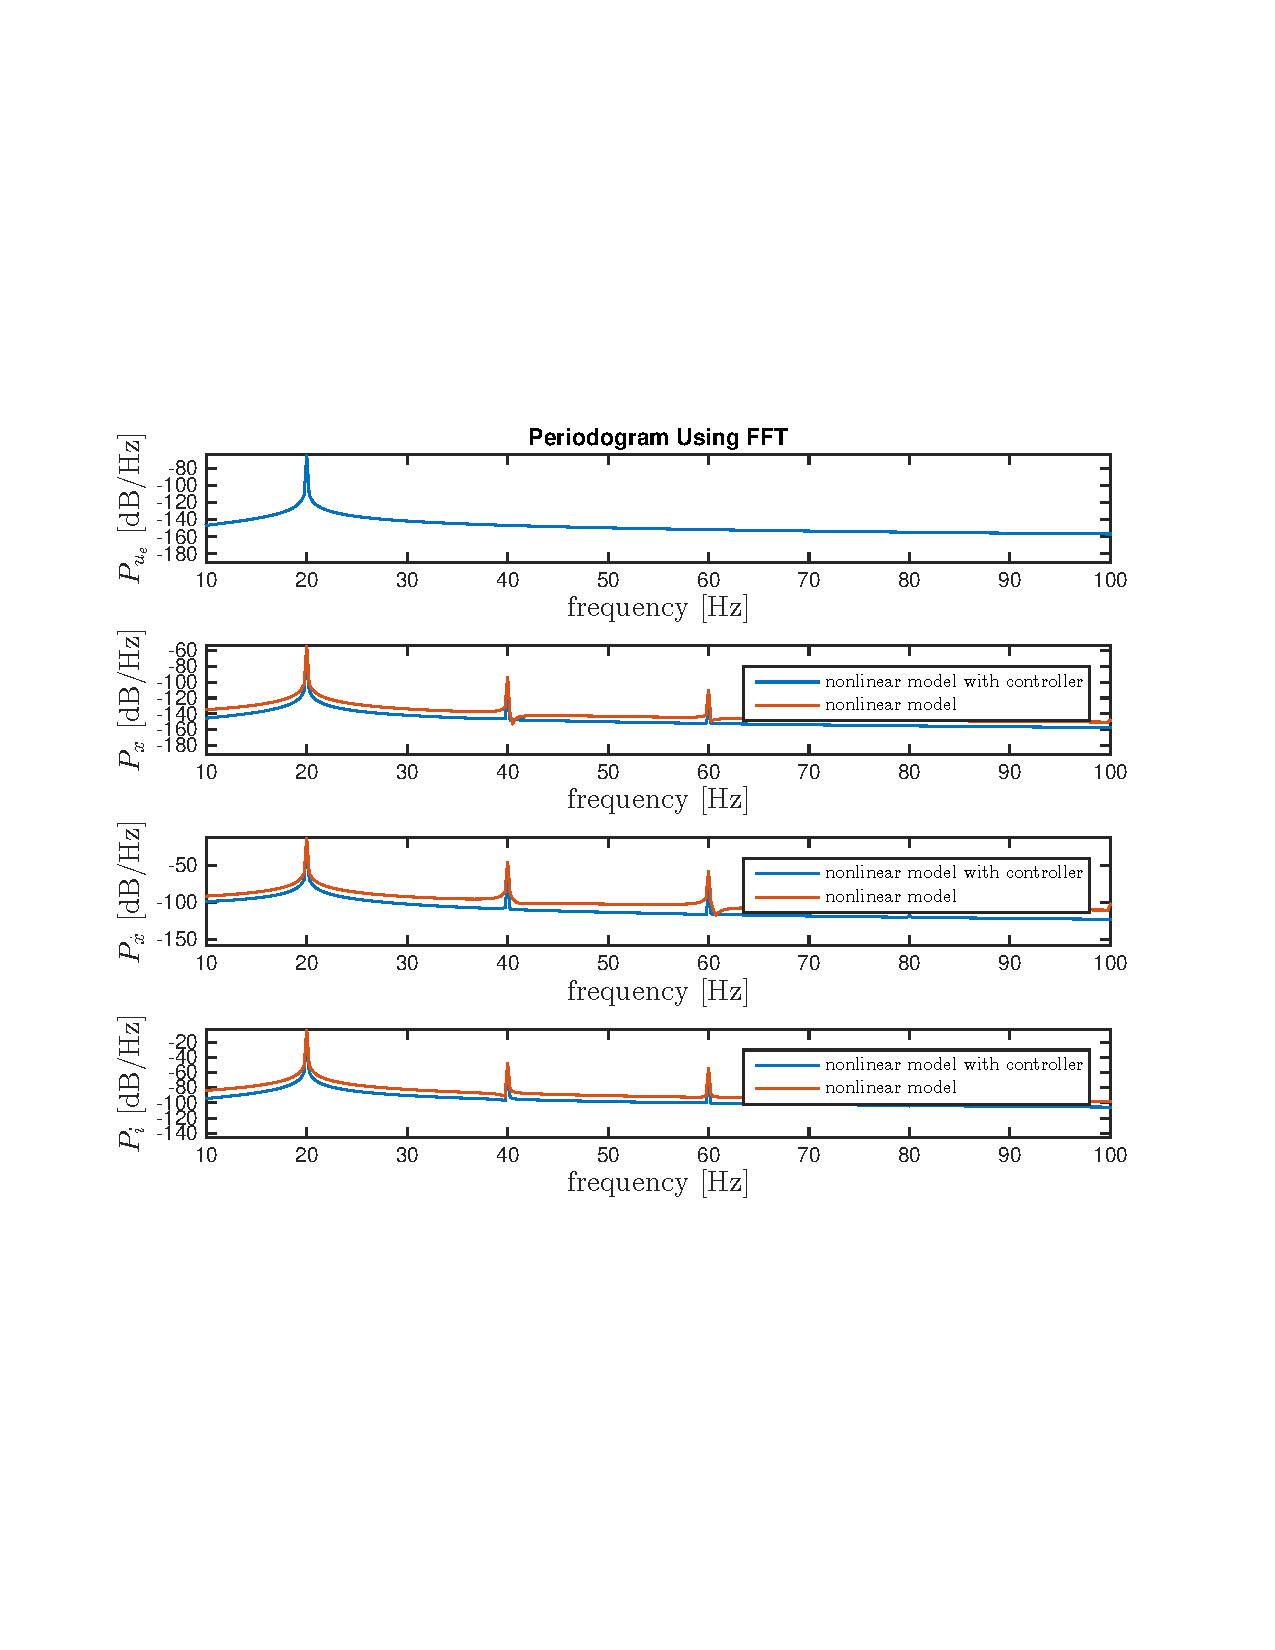
\includegraphics[trim=0cm 7cm 0cm 7cm, clip=true, totalheight=0.35\textheight, angle=0]{figures/p17freq.pdf}
 \caption{PSD of $u_e$ and the states response to $x_{ref}$ with $Ax = 0.0005\ m$ using the controller on the nonlinear model.}
 \label{fig:p17freq}
\end{figure}

As we can see figure \ref{fig:p17time}, the reference is well tracked with a delay $\tau = 0.0016\ s$. Moreover, $u_e$ has also been plotted figure \ref{fig:p17time} and we can notice that $\max(u_e) \simeq 2 < 40\ V$, which respects the condition of the maximum voltage. The simulation has also been run with $Ax = 0.001\ m$ and $\max(u_e) \simeq 4 < 40\ V$ too ($\tau = 0.0011\ s$).

Also, we can see figure \ref{fig:p17freq} that the harmonic distortion is attenuated. Indeed, we can see tab \ref{tabTHD} that the percentage of the \textit{Total Harmonic Distortion (THD)} has decreased a lot, there is only 2 to 4\% of the initial THD left. Moreover, the distortion levels of the second and third harmonic ($d_2$, $d_3$) have decreased a lot too (see table \ref{tabTHD}). Therefore, we can say that the controller succeeded in attenuating the harmonic distortion.

\begin{table}[H]
 \centering 
\begin{tabular}{|l|c|c|r|}
  \hline
   & with controller (Ax = 0.0005 m) & with controller (Ax = 0.001 m) & without controller \\
  \hline
  THD & 0.0470 \% & 0.0966 \% & 2.4350 \%\\
	\hline
  d2 & 0.0467 \%& 0.0930 \% & 2.3735 \%\\
	\hline
	d3 & 0.0056 \%& 0.0261 \% & 0.5432 \%\\
  \hline
\end{tabular}
\caption{THD, d2 an d3 of the coil velocity with the nonlinear model with and without controller (include the first 5 harmonics after the fundamental frequency fc = 20 $Hz$)}
	\label{tabTHD}
	\end{table}